\documentclass[12pt]{article}
\usepackage[left=0.75in,right=0.75in,top=0.75in,bottom=0.75in,
            footskip=0.25in]{geometry}
\usepackage{graphicx,float,hyperref} 
\usepackage{amsmath,amsthm,amssymb,amsfonts,geometry,mathtools,enumerate,bbm}
\usepackage{algpseudocode}
\usepackage{fancyvrb}
\usepackage{xcolor}
 
\theoremstyle{plain}
\newtheorem{theorem}{Theorem}[section]
\newtheorem{lemma}[theorem]{Lemma}
\newtheorem{proposition}[theorem]{Proposition}
\newtheorem{corollary}[theorem]{Corollary}
\newtheorem{conjecture}[theorem]{Conjecture}
\newtheorem{question}[theorem]{Question}
\newtheorem{property}[theorem]{Property}

\theoremstyle{definition}
\newtheorem{definition}[theorem]{Definition}
\newtheorem{problem}[theorem]{Problem}
\newtheorem{example}[theorem]{Example}
\newtheorem{examples}[theorem]{Examples}


\theoremstyle{remark}
\newtheorem{remark}[theorem]{Remark}
\newtheorem{claim}[theorem]{Claim}
\newtheorem{observation}[theorem]{Observation}
\newtheorem{exercise}[theorem]{Exercise}
\newtheorem{exercises}[theorem]{Exercises}

\newcommand{\Bin}{\ensuremath{\textrm{Bin}}}
\newcommand{\Unif}{\ensuremath{\textrm{Unif}}}
 
 
\newcommand{\N}{\mathbb{N}}
\newcommand{\Z}{\mathbb{Z}}
\newcommand{\C}{\mathbb{C}}
\newcommand{\R}{\mathbb{R}}
\newcommand{\Q}{\mathbb{Q}}
\newcommand{\F}{\mathbb{F}}


\DeclarePairedDelimiter{\ceil}{\lceil}{\rceil}
\DeclarePairedDelimiter{\floor}{\lfloor}{\rfloor}
 
% \newenvironment{problem}[2][Problem]{\begin{trivlist}
% \item[\hskip \labelsep {\bfseries #1}\hskip \labelsep {\bfseries #2.}]}{\end{trivlist}}
%If you want to title your bold things something different just make another thing exactly like this but replace "problem" with the name of the thing you want, like theorem or lemma or whatever
 
\begin{document}
 
%\renewcommand{\qedsymbol}{\filledbox}
%Good resources for looking up how to do stuff:
%Binary operators: http://www.access2science.com/latex/Binary.html
%General help: http://en.wikibooks.org/wiki/LaTeX/Mathematics
%Or just google stuff
 
\title{Math 130B}
\author{Liam Hardiman}

\maketitle

\begin{abstract}
    I'm writing these lecture notes for UC Irvine's Math 130B course, taught in the summer of 2022.
    This is a five-ish week course where I plan to get through chapters 6-8 of Ross' book \cite{Ross}.
    The class structure consists of a two hour lecture followed by a one hour discussion section three days a week.
    I'm aiming to get through one or two sections of the book per lecture with a midterm soon after chapter 6, maybe partway into chapter 7.

\end{abstract}


\tableofcontents


\section{Jointly Distributed Random Variables}
Many of life's more interesting problems are multifaceted.
For example, in a clinical trial for a cholesterol drug, we might be interested in a patient's cholesterol levels \emph{and} how many hours they exercise each week.
Or if we're interested in California's gas consumption, we'd be interested in how much gas each station sells \emph{and} its price of gas.

In this section, we address how to look at more than one random variable at the same time.


\subsection{Joint Distribution Functions}

Remember that we can define the \emph{probability mass function} of a discrete random variable $X$ to be the function that takes in a value and returns the probability that $X$ attains that value.
\[
    p(a) = \Pr[X = a].
\]

\begin{examples}
\begin{enumerate}[(a)]
    \item Suppose we roll a pair of dice and $X$ is the sum of the values shown.
    Then $X$ can take any integer value between 2 and 12 and its probability mass function is
    \begin{align*}
        p(2) = p(12) &= \frac{1}{36} & p(3) = p(11)&= \frac{2}{36}\\
        p(4) = p(10) &= \frac{3}{36} & p(5) = p(9)&= \frac{4}{36}\\
        p(6) = p(8) &= \frac{5}{36} & p(7) &= \frac{6}{36}.
    \end{align*}

    \item Suppose Alice is communicating with Bob by sending him bits (0's or 1's) one by one.
    Suppose each bit Alice sends has probability $p$ of successfully getting to Bob and each transmission is independent of the others.
    If $X$ is the first time a bit fails to transmit properly (maybe there's too much noise on the channel), then $X$ is a geometric random variable with probability mass function
    \[
        p(n) = p^{n-1}(1-p).
    \]
\end{enumerate}
\end{examples}

Situations naturally arise where we might want to look at two discrete random variables at the same time.
For example, if we roll two dice and $X$ is the smaller roll and $Y$ is the larger one, can we define an analogue of the probability mass function?

\begin{definition}
    Suppose $X$ and $Y$ are two discrete random variables taking values in the sets $A$ and $B$, respectively.
    Then their \emph{joint probability mass function} is the function $p: A\times B\to [0,1]$ defined by
    \[
        p(a,b) = \Pr[X = a, Y = b].
    \]
\end{definition}

\begin{example}
    Say we roll two dice and $X$ is the largest value shown and $Y$ is the sum of the two values.
    Let's compute a few values of the joint probability mass function of $X$ and $Y$.
    We have
    \begin{align*}
        p(3, 5) &= \Pr[X = 3, Y = 5]\\
        &= \Pr[\{(3,2), (2,3)\}]\\
        &= \frac{2}{36}.
    \end{align*}
    This is because the only way for the largest value to be 3 and the sum to be 5 is for one of the dice to show 2 and the other to show 3.
    We also have
    \[
        p(1, 8) = 0
    \]
    since there's no way for two dice to sum to 8 and the largest value be a 1.
\end{example}

How does the joint mass function of $X$ and $Y$ relate to the \emph{marginal} probability mass functions?
Well if we just specify that $X = a$, then we haven't put any restrictions on $Y$.
This gives us
\begin{equation}
\begin{split}
    p_X(a) &= \Pr[X= a]\\
    &= \Pr[X = a, Y<\infty]\\
    &= \sum_{y\in B}\Pr[X = a, Y = y]\\
    &= \sum_{y\in B}p(a, y).
\end{split}
\end{equation}

Similarly, we have
\[
    p_Y(b) = \sum_{x\in A}p(x, b).
\]

\begin{example}
    Say 100 people are asked for their handedness (right-handed or left-handed) and sex (male or female).
    The survey produces the following table.
    \begin{center}
    \begin{tabular}{|c || c | c|}
        \hline
           & L & R\\
        \hline
         M & 4 & 44\\
         F & 9 & 43\\
         \hline
    \end{tabular}
    \end{center}
    If we randomly select one of these people and let $X$ be their sex and $Y$ be their handedness, then we can obtain the joint probability mass function by just reading off values from the table.
    \begin{align*}
        p(M, L) &= 4/100  &  p(M, R) &= 44/100\\
        p(F, L) &= 9/100  &  p(F, R) &= 43/100.
    \end{align*}
    Let's compute the marginal probability mass functions.
    For $X$ we have
    \begin{align*}
        p_X(M) &= p(M, L) + p(M, R) = \frac{4}{100} + \frac{44}{100} = \frac{48}{100}\\
        p_X(F) &= p(F, L) + p(F, R) = \frac{9}{100} + \frac{43}{100} = \frac{52}{100}.
    \end{align*}
    For $Y$ we have
    \begin{align*}
        p_Y(L) &= p(M, L) + p(F, L) = \frac{4}{100} + \frac{9}{100} = \frac{13}{100}\\
        p_Y(R) &= p(M, R) + p(F, R) = \frac{44}{100} + \frac{43}{100} = \frac{87}{100}.
    \end{align*}
\end{example}


\begin{example}
    In the previous example we determined the marginal mass function from the joint mass function.
    Can we go the other way?
    That is, if we know the marginal mass functions for $X$ and $Y$, can we determine the joint mass function?
    Well here's another possible outcome of the same survey from the previous example.
    \begin{center}
    \begin{tabular}{|c || c | c|}
        \hline
           & L & R\\
        \hline
         M & 3 & 45\\
         F & 10 & 42\\
         \hline
    \end{tabular}
    \end{center}
    It's easy to check that we get the same marginal mass functions in this modified example.
    So if we started with the marginals, how would we know whether the survey outcome was given by this table or the previous one?
    Since we can't really tell, it looks like the marginals don't determine the joint.

    Let's be a little more specific.
    Suppose the marginals are specified by these equations
    \begin{align*}
        p_X(M) &= p_{ML} + p_{MR} = 48/100\\
        p_X(F) &= p_{FL} + p_{FR} = 52/100\\
        p_Y(L) &= p_{ML} + p_{FL} = 13/100\\
        p_Y(R) &= p_{MR} + p_{FR} = 87/100.
    \end{align*}
    Finding the joint mass function amounts to solving this system for the variables $p_{ML}, p_{MR}, p_{FL}, p_{FR}$.
    This is a linear system with four equations and four unknowns, so this sounds promising.
    The corresponding matrix equation is
    \[
        \begin{bmatrix}
            1 & 1 & 0 & 0\\
            0 & 0 & 1 & 1\\
            1 & 0 & 1 & 0\\
            0 & 1 & 0 & 1
        \end{bmatrix}
        \begin{bmatrix}
            p_{ML}\\
            p_{MR}\\
            p_{FL}\\
            p_{FR}
        \end{bmatrix}
        =
        \begin{bmatrix}
            48/100\\
            52/100\\
            13/100\\
            87/100
        \end{bmatrix}.
    \]
    If we go through the usual procedure of row-reduction, the coefficient matrix reduces to
    \[
        \begin{bmatrix}
            1 & 0 & 0 &-1\\
            0 & 1 & 0 & 1\\
            0 & 0 & 1 & 1\\
            0 & 0 & 0 & 0
        \end{bmatrix}.
    \]
    This matrix doesn't have full rank, so the system does \emph{not} have a unique solution.
    In particular, there isn't just one joint mass function corresponding to these marginals.
\end{example}


Let's move on to continuous random variables.
Remember that every (real-valued) random variable $X$ gives us a function $F_X:\R\to [0,1]$ called its \emph{(cumulative) distribution function}:
\begin{equation}
    F_X(t) = \Pr[X \leq t].
\end{equation}
Likewise, if we have two random variables $X$ and $Y$, we can define their \emph{joint (cumulative) distribution function}.
\begin{definition}
    Let $X$ and $Y$ be two random variables.
    Then their \emph{joint cumulative distribution function}, $F: \R^2\to [0,1]$ is defined by
    \[
        F(a,b) = \Pr[X\leq a, Y\leq b].
    \]
    If there's any possibility for ambiguity, we might write $F_{X,Y}$ to remind us that $F$ is the cumulative distribution function for $X$ and $Y$.
\end{definition}

How is the joint distribution function related to the \emph{marginal} distribution functions of $X$ and $Y$?
Like in the discrete case, if we just specify that $X\leq a$, then we haven't put any restrictions on $Y$.
This gives us
\begin{equation}\label{marginal1}
\begin{split}
    F_X(a) &= \Pr[X\leq a]\\
    &= \Pr[X \leq a, Y<\infty].
\end{split}
\end{equation}
Now the events $\{X\leq a, Y\leq t\}$ form an increasing sequence of events as $t$ increases.
That is, if $t_1 < t_2$, then we have the inclusion
\[
    \{X\leq a, Y\leq t_1\} \subseteq \{X\leq a, Y\leq t_2\}.
\]
This is helpful because probabilities play nicely with increasing (or decreasing) sequences of events.
Namely, if $E_1 \subseteq E_2 \subseteq \cdots$ is an increasing sequence of events, then
\[
    \Pr\left[\bigcup_{n=1}^\infty E_n\right] = \lim_{n\to \infty}\Pr[E_n].
\]
Using this, (\ref{marginal1}) becomes
\begin{align*}
    F_X(a) &= \Pr[X \leq a, Y< \infty]\\
    &= \Pr\left[ \bigcup_{b\geq 0}\{X\leq a, Y\leq b\}\right]\\
    &= \lim_{b\to \infty}\Pr\left[X\leq a, Y\leq b\right]\\
    &= \lim_{b\to \infty}F(a,b)
\end{align*}

The same idea tells us that
\[
    F_Y(b) = \lim_{a\to \infty}F(a, b).
\]

When working with continuous random variables, we often work with their \emph{density functions}.
Specifically, if $X$ is a continuous random variable, there is some function $f$ such that for (pretty much)\footnote{Technically, $B$ needs to be what's called a \emph{measurable} set. Pretty much any set you'd care about is measurable, but we need this restriction for the theory to hold up.} any set $B\subseteq \R$,
\[
    \Pr[X\in B] = \int_Bf(x)\ dx.
\]
Here's the analogue for multiple variables.

\begin{definition}
    Let $X$ and $Y$ be continuous random variables.
    We say $X$ and $Y$ have a \emph{continuous joint distribution} if there is some function $f: \R^2\to [0,1]$ such that
    \[
        \Pr[(X,Y)\in C] = \int_Cf(x,y)\ dydx.
    \]
    In this case, we call $f$ the \emph{joint probability density function (pdf)} of $X$ and $Y$.
\end{definition}

In the discrete case we were able to start with a joint mass function and sum over one of the variables to obtain the marginal of the other variable.
Here's the analogue for continuous random variables.

\begin{proposition}
    Suppose $X$ and $Y$ are jointly continuous random variables with joint probability density function $f$.
    Then $X$ and $Y$ are continuous random variables with density functions
    \begin{align*}
        f_X(x) &= \int_\R f(x,y)\ dy\\
        f_Y(y) &= \int_\R f(x,y)\ dx,
    \end{align*}
    respectively.
\end{proposition}
\begin{proof}
    Suppose $B\subseteq \R$ is measurable (don't worry too much about this assumption).
    Then
    \begin{align*}
        \Pr[X\in B] &= \Pr[X\in B, Y\in \R]\\
        &= \int_B\left(\int_\R f(x,y)\ dy\right)dx.
    \end{align*}
    So the function
    \[
        f_X(x) = \int_\R f(x,y)\ dy
    \]
    plays the role of the density function for $X$.
    The same idea gives the density function for $Y$.
\end{proof}

\begin{example}\label{triangle density}
    Let $X$ and $Y$ be random variables with joint pdf
    \[
        f(x,y) = \begin{cases}
            kxy,&\text{if }x,y\geq 0,\ x+y \leq 1\\
            0,&\text{otherwise,}
        \end{cases}
    \]
    where $k$ is some constant.

    Let's determine the actual value of $k$.
    We must have the following
    \[
        1 = \Pr[(X,Y) \in \R^2] = \int_{\R^2}f(x, y)\ dydx,
    \]
    so we're just going to have to evaluate this integral and then solve for $k$.
    It's usually a good idea to draw the region in question when computing double integrals like this.
    % \begin{center}
    %     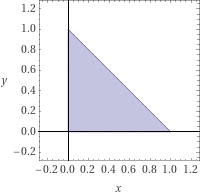
\includegraphics[scale=1]{1-1region.png}
    % \end{center}
    \begin{figure}[h]
    \centering        
        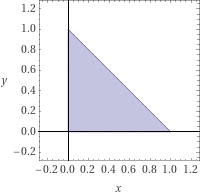
\includegraphics[scale=1]{1-1region.png}
        \caption{The joint density function $f(x,y)$ is nonzero in the shaded region.}
    \end{figure}
    As $x$ ranges from 0 to 1, $y$ ranges from 0 to $1-x$.
    To see this, draw a vertical slice upwards from any point on the $x$-axis until it intersects the line $x+y=1$.
    Our integral then becomes
    \begin{align*}
        k\int_0^1\int_0^{1-x}xy\ dydx &= k\int_0^1x\left[\frac{1}{2}y^2\right]_{y=0}^{1-x}dx\\
        &= \frac{k}{2}\int_0^1x(1-x)^2\ dx\\
        &= \frac{k}{2}\left[\frac{1}{4}x^4-\frac{2}{3}x^3 + \frac{1}{2}x^2\right]_{x=0}^{x=1}\\
        &= k/24.
    \end{align*}
    Since this expression must be equal to 1, we have $k=24$.

    Now let's compute the marginal pdf's of $X$ and $Y$.
    To get the marginal for $X$, we ``integrate out the $y$.''
    For any fixed $x$, the value of $y$ ranges between 0 and $1-x$, so we have
    \[
        f_X(x) = \int_{\R}f(x,y)\ dy = \int_0^{1-x}kxy\ dy = \frac{k}{2}x(1-x)^2 = 12x(1-x)^2.
    \]
    Similarly, for any fixed $y$, the value of $x$ ranges between 0 and $1-y$.
    \[
        f_Y(y) = \int_{\R}f(x,y)\ dx = \int_0^{1-y}kxy\ dx = \frac{k}{2}y(1-y)^2 = 12y(1-y)^2.
    \]
\end{example}

\begin{example}
    The joint density function of $X$ and $Y$ is given by
    \[
        f(x,y) = \begin{cases}
            2e^{-x}e^{-2y},&\text{if }0<x<\infty, 0<y<\infty\\
            0,&\text{otherwise.}
        \end{cases}
    \]

    Let's compute $\Pr[X>1, Y<1]$.
    To compute the probability of \emph{any} event, we simply integrate the joint density function over that event.
    In this case we have
    \begin{align*}
        \Pr[X > 1, Y< 1] &= \int_0^1\int_1^\infty2e^{-x}e^{-2y}\ dxdy\\
        &= \int_0^12e^{-2y}\left[-e^{-x}\right]_{x=1}^{x=\infty}dy\\
        &= 2e^{-1}\int_0^1e^{-2y}dy\\
        &= e^{-1}(1-e^{-2}).
    \end{align*}
\end{example}

In the case of a single random variable, the density and distribution functions are related by differentiation.
That is, if $X$ has density function $f$ and distribution function $F$, then
\[
    f(x) = \frac{d}{dx}F(x).
\]
The multivariable analogue is what you would probably expect.
If $X$ and $Y$ are jointly continuous with density function $f(x,y)$ and distribution function $F(x,y)$, then we have by Fubini's theorem
\begin{equation}\label{derivative of distribution is density}
    f(x,y) = \frac{\partial^2}{\partial x \partial y}F(x,y) = \frac{\partial^2}{\partial y\partial x}F(x,y).
\end{equation}
We aren't going to angst over the proof here, but this technically only holds for the values of $(x,y)$ where the partial derivatives are defined and continuous.










\subsection{Independent Random Variables}
Remember that we said that two \emph{events} $A$ and $B$ are independent if
\[
    \Pr[A\cap B] = \Pr[A]\cdot \Pr[B].
\]
We can carry this definition over to random variables.
\begin{definition}
    Let $X$ and $Y$ be random variables.
    Then $X$ and $Y$ are \emph{independent} if for any measurable sets $A$ and $B$ we have
    \[
        \Pr[X\in A, Y\in B] = \Pr[X\in A]\cdot \Pr[Y\in B].
    \]
\end{definition}

Let's show that this definition plays nicely with the machinery we defined in the previous section.

\begin{proposition}
    The discrete random variables $X$ and $Y$, taking values in $\mathcal X$ and $\mathcal Y$, respectively, are independent if and only if
    \begin{equation}\label{discrete indep}
        p(x,y) = p_X(x)p_Y(y)
    \end{equation}
    for all $x\in \mathcal X$ and $y\in \mathcal Y$.
\end{proposition}
\begin{proof}
    First let's suppose that $X$ and $Y$ are independent.
    Then we can consider the singleton sets $\{x\}$ and $\{y\}$ for any $x\in \mathcal X$, $y\in \mathcal Y$.
    \[
        p(x,y) = \Pr[X = x, Y=y] = \Pr[X=x]\Pr[Y=y] = p_X(x)p_Y(y).
    \]

    Now suppose that equation (\ref{discrete indep}) holds.
    Then for any sets $A\subseteq \mathcal X$ and $B\subseteq \mathcal Y$ we have
    \begin{align*}
        \Pr[X\in A, Y\in B] &= \sum_{x\in A, y\in B}p(x,y)\\
        &= \sum_{x\in A}p_X(x)\sum_{y\in B}p_Y(y)\\
        &= \Pr[X\in A]\Pr[Y\in B],
    \end{align*}
    so $X$ and $Y$ are independent.
\end{proof}


\begin{example}
    Suppose we perform $n+m$ independent trials, each having common success probability $p$.
    Let $X$ be the number of successes in the first $n$ trials and let $Y$ be the number of successes in the next $m$ trials.
    Are $X$ and $Y$ independent?
    Intuitively, knowing what happens in the first $n$ trials shouldn't tell us anything about what happens in the next $m$ trials, so we hope that $X$ and $Y$ are independent.
    Indeed, we have
    \[
        \Pr[X = x, Y=y] = \binom{n}{x}p^x(1-p)^{n-x}\binom{m}{y}p^y(1-p)^{m-y}= \Pr[X=x]\Pr[Y=y].
    \]

    Let's define a new random variable $Z$ to be the total number of successes in all $m+n$ trials.
    Are $X$ and $Z$ independent?
    Well if we know there are some successes in the first $n$ trials, then we definitely know that there are at least that many successes in total, so we suspect that these aren't independent.
    We have
    \begin{align*}
        p(x,z) &= \Pr[x\text{ successes in the first $n$ trials, $z$ successes total}]\\
        &= \Pr[x\text{ successes in the first $n$ trials, $z-x$ successes in the next $m$ trials}]\\
        &= \binom{n}{x}p^x(1-p)^{n-x}\binom{m}{z-x}p^{z-x}(1-p)^{m-z+x}.
    \end{align*}
    However,
    \begin{align*}
        p_X(x) &= \binom{n}{x}p^x(1-p)^{n-x}\\
        p_Z(z) &= \binom{n+m}{z}p^z(1-p)^{n+m-z}.
    \end{align*}
    It's easily seen that the product of these two quantities does not match up with the previous quantity, so $X$ and $Z$ are \emph{not} independent.
\end{example}

So we can check to see if two discrete random variables are independent by looking at their mass functions.
What about continuous random variables?
We should think of a discrete random variable's mass function as being analogous to a continuous random variable's density function, and this informs the next proposition.

\begin{proposition}
    If $X$ and $Y$ are continuous random variables, then they are independent if and only if
    \[
        f(x,y) = f_X(x)f_Y(y).
    \]
\end{proposition}
\begin{proof}
    Suppose $X$ and $Y$ are independent.
    This is really a statement about \emph{distribution} functions, not density functions, so we have
    \begin{equation}\label{continuous indep}
        \Pr[X\leq x, Y\leq y] = \Pr[X\leq x]\Pr[Y\leq y],
    \end{equation}
    which is equivalent to
    \[
        F(x,y) = F_X(x)F_Y(y).
    \]
    Now let's take the mixed $x$ and $y$ partial derivatives of both sides to obtain
    \[
        \frac{\partial^2}{\partial x\partial y}F(x,y) = \frac{\partial^2}{\partial x\partial y}\big(F_X(x)F_Y(y)\big) = \frac{\partial}{\partial x}F_X(x)\frac{\partial}{\partial y}F_Y(y).
    \]
    We arrived at the last equality using the fact that $F_X(x)$ is constant with respect to $y$ and $F_Y(y)$ is constant with respect to $x$.
    Since differentiation distributions gives us densities, we have
    \[
        f(x,y) = f_X(x)f_Y(y)
    \]
    as desired.

    Conversely, suppose that equation (\ref{continuous indep}) holds.
    We pretty much copy the proof of the previous proposition with integrals in place of sums.
    For any sets $A$ and $B$ we have
    \begin{align*}
        \Pr[X\in A, Y\in B] &= \int_A\int_Bf(x,y)\ dydx\\
        &= \int_Af_X(x)\ dx\int_Bf_Y(y)\ dy\\
        &= \Pr[X\in A]\Pr[Y\in B].
    \end{align*}
\end{proof}

So we have have independence if our joint density (or mass) function factors into the product of the marginals.
We can actually say more -- factoring into \emph{any} product of functions, each depending on just one variable, is enough.
\begin{proposition}
    Let $X$ and $Y$ be continuous random variables.
    Then $X$ and $Y$ are independent if and only if the joint density function can be factored as
    \begin{equation}\label{joint factors}
        f(x,y) = h(x)g(y)
    \end{equation}  
    for some functions $g$ and $h$.
\end{proposition}
\begin{proof}
    If $X$ and $Y$ are independent, then the previous proposition tells us that we can just take $g = f_X$ and $h = f_Y$.

    Conversely, suppose that $f(x,y) = h(x)g(y)$.
    Then
    \begin{align*}
        1 &= \int_\R\int_\R f(x,y)\ dxdy\\
        &= \int_\R h(x)\ dx\cdot \int_\R g(y)\ dy.
    \end{align*}
    But these last two integrals have to each be equal to some constants, $c_1$ and $c_2$, respectively.
    We also have
    \begin{align*}
        f_X(x) &= \int_\R f(x,y)\ dy\\
        &= \int_\R h(x)g(y)\ dy\\
        &= c_1 h(x).
    \end{align*}
    Similarly, $f_Y(y) = c_2g(y)$.
    Putting it all together, we have
    \begin{align*}
        f_X(x)f_Y(y) &= c_1h(x)\cdot c_2g(y)\\
        &= (c_1c_2)h(x)g(y)\\
        &= f(x,y).
    \end{align*}
\end{proof}

\begin{example}
Suppose $X$ and $Y$ are jointly continuous random variables with joint density
    \[
        f(x,y) = \begin{cases}
            kxy,&\text{if }(x,y)\in [0,1]^2\\
            0,&\text{otherwise.}
        \end{cases}
    \]
Are $X$ and $Y$ independent?
They'd definitely be independent it we could factor the joint density, but how does the piecewise nature of the density play into this?
Let's define the \emph{indicator function} for the set our density actually lives on.
That is, let $I(x,y)$ be defined by
\[
    I(x,y) = \begin{cases}
        1,&\text{if }(x,y)\in [0,1]^2\\
        0,&\text{otherwise.}
    \end{cases}
\]
That is, $I(x,y)$ indicates whether or not $(x,y)$ lives in the set $[0,1]^2$, the unit square in $\R^2$.
We go through the trouble of defining this function because we can use it to write our density as
\[
    f(x,y) = kxy\cdot I(x,y).
\]
The $kxy$ part is clearly a product of a function of only $x$ with a function of only $y$.
If we could factor the indicator function $I$ into functions of just $x$ and just $y$, then we will have shown independence.
Our ability to do this is going to come down to the nature of the set $[0,1]^2$.
Notice that $(x,y)\in [0,1]^2$ if and only if both coordinates live in $[0,1]$.
That is, if we define $\tilde{I}(x)$ by
\[
    \tilde{I}(x) = \begin{cases}
        1,&\text{if }x\in [0,1]\\
        0,&\text{otherwise,}
    \end{cases}
\]
then we have $I(x,y) = \tilde{I}(x)\tilde{I}(y)$, so our joint density factors as
\[
    f(x,y) = (kx\cdot \tilde{I}(x))(y\cdot \tilde{I}(y)),
\]
so $X$ and $Y$ are independent.
\end{example}

\begin{example}
Suppose $X$ and $Y$ are jointly continuous random variables with joint density
    \[
        f(x,y) = \begin{cases}
            kxy,&\text{if }x,y\geq 0, x+y\leq 1\\
            0,&\text{otherwise.}
        \end{cases}
    \]
Are $X$ and $Y$ independent?
This density looks a lot like the one from the previous exercise.
The difference here is that $f(x,y)$ behaves like $kxy$ on a different set this time.
Now $f$ lives on a triangle in the first quadrant rather than an axis-aligned square.
Proceeding in the same way as before, if we define
\[
    I(x,y) = \begin{cases}
        1,&\text{if }x,y\geq 0, x+y\leq 1\\
        0,&\text{otherwise,}
    \end{cases}
\]
Then we still have $f(x,y) = kxy\cdot I(x,y)$ like before.
Can we still factor it?
Well if we specify the $x$ coordinate to live between 0 and 1, then the $y$ coordinate needs to satisfy $0\leq y\leq 1-x$.
If we define the functions $I_1$ and $I_2$ by
\[
    I_1(x) = \begin{cases}
        1,&\text{if }x\in [0,1]\\
        0,&\text{otherwise,}
    \end{cases} \qquad
    I_2(x,y) = \begin{cases}
        1,&\text{if }0\leq y\leq 1-x\\
        0,&\text{otherwise,}
    \end{cases}
\]
then we do get the factorization
\[
    f(x,y) = kxy \cdot I_1(x)\cdot I_2(x,y),
\]
but this isn't helpful since $I_2(x,y)$ is a function of both $x$ and $y$.

This is \emph{not} a proof that $X$ and $Y$ aren't independent.
For all we know, there's some weird factorization of $f(x,y)$ we just haven't found yet.
Let's approach it a bit differently.
This is the same density from Example \ref{triangle density} and we found the marginal density functions to be
\[
    f_X(x) = \begin{cases}
        (k/2)x(1-x)^2,&\text{if }0\leq x \leq 1\\
        0,&\text{otherwise,}
    \end{cases}\qquad
    f_Y(y) = \begin{cases}
        (k/2)y(1-y)^2,&\text{if }0\leq y \leq 1\\
        0,&\text{otherwise.}
    \end{cases}
\]
Notice that we do \emph{not} have that $f(x,y) = f_X(x)f_Y(y)$ for all $x,y$ where these three functions are defined, so $X$ and $Y$ are \emph{not} independent.
\end{example}










\subsection{Sums of Independent Random Variables}
Say we have two real-valued random variables $X$ and $Y$.
We'll assume they're discrete for now.
Their sum $Z=X+Y$ is clearly a random variable as well.
How do the mass functions of $X$ and $Y$, $p_X$ and $p_Y$, and the joint mass function $p$ relate to the mass function of $X+Y$?
Well $p_Z(z) = \Pr[Z = z]$ and we can break the event $\{Z = z\}$ into the events
\[
    \{Z = z\} = \bigcup_{x}\{X = x, Y = z-x\}.
\]
To see this, note that in order for $X+Y = z$ to be true, $X$ can be anything so long as $Y = z-X$.
Moreover, these events are clearly disjoint since $X$ and $Y$ can only take one value at a time.
Since the probability of a \emph{disjoint} union is just the sum of the probabilities of the constituent events, we have
\[
    p_Z(z) = \sum_x \Pr[X = x, Y= z-x] = \sum_x p(x, z-x).
\]
Now if $X$ and $Y$ are independent, the joint density factors as $p(x,y) = p_X(x)p_Y(y)$ and we've proven the following proposition.
\begin{proposition}
    If $X$ and $Y$ are discrete random variables, then the probability mass function of $Z = X+Y$ is
    \[
        p_Z(z) = \sum_x p_X(x)p_Y(z-x).
    \]
\end{proposition}

\begin{example}
    Suppose $X$ and $Y$ are independent random variables, both taking values in $\{1, 2, \ldots, n\}$ uniformly at random (if $n=6$, then you can think $X$ and $Y$ as the outcomes of dice rolls).
    If we set $Z = X+Y$, then the previous proposition tells us that
    \[
        p_Z(z) = \sum_{j = 1}^np_X(j)p_Y(z-j).
    \]
    Now it might be tempting to just set $p_X(j)$ and $p_Y(z-j)$ to $1/n$.
    If this were the case, then we would have $p_Z(z) = 1/n$ for each $z$.
    But this definitely doesn't line up with our intuition -- when we roll two dice, some outcomes are more likely than others (there's only one way to roll a 2, but six ways to roll a 7).
    The problem is that $p_Y(z-j)$ isn't always $1/n$.
    Indeed, if $z-j < 1$, then $Y$ never takes the value $z-j$.

    We can fix this by looking at the conditions that make $p_X(j)$ and $p_Y(z-j)$ \emph{both} positive.
    In order for this to happen, we need $1\leq j\leq n$ \emph{and} $1\leq z-j\leq n$ to both hold.
    Isolating $j$ gives
    \[
        z-n \leq j\leq z-1 \qquad\text{and}\qquad 1\leq j\leq n.
    \]
    If $z$ is between $2$ and $n$ this becomes
    \[
        p_Z(z) = \sum_{j=1}^{z-1}p_X(j)p_Y(z-j) = \sum_{j=1}^{z-1}\frac{1}{n^2} = \frac{z-1}{n^2}. 
    \]
    On the other hand, if $z$ is between $n+1$ and $2n$ we have
    \[
        p_Z(z) = \sum_{j=z-n}^n p_X(j)p_Y(z-j) = \sum_{j=z-n}^n\frac{1}{n^2} = \frac{2n-z+1}{n^2}.
    \]
    So in total we have
    \[
        p_Z(z) = \begin{cases}
            (z-1)/n^2,&\text{if }2\leq z \leq n\\
            (2n-z+1)/n^2,&\text{if }n+1\leq z\leq 2n.
        \end{cases}
    \]
    Importantly, we have that the sum of two uniform random variables is \emph{not} another uniform random variable.
\end{example}

\begin{example}\label{sum of Poissons}
    If $X$ and $Y$ are independent Poisson random variables with respective parameters $\lambda_1$ and $\lambda_2$, let's compute the distribution of $X+Y$.

    We have that
    \begin{align*}
        \Pr[X+Y = n] &= \sum_{k=0}^n\Pr[X = k, Y = n-k]\\
        &= \sum_{k=0}^n\Pr[X=k]\Pr[Y=n-k]\\
        &= \sum_{n=0}^n e^{-\lambda_1}\frac{\lambda_1^k}{k!}e^{-\lambda_2}\frac{\lambda_2^{n-k}}{(n-k)!}\\
        &= e^{-(\lambda_1+\lambda_2)}\sum_{k=0}^n\frac{\lambda_1^k\lambda_2^{n-k}}{k!(n-k)!}.
    \end{align*}
    Now the sum at the end should remind us of the binomial theorem since it has a product of two terms whose powers sum to $n$.
    We almost have the correct binomial coefficient too.
    We just need to multiply and divide by $n!$.
    \begin{align*}
        \Pr[X+Y = n] &= e^{-(\lambda_1+\lambda_2)}\sum_{k=0}^n\frac{\lambda_1^k\lambda_2^{n-k}}{k!(n-k)!}\\
        &= \frac{e^{-(\lambda_1+\lambda_2)}}{n!} \sum_{k=0}^n\frac{n!}{k!(n-k)!}\lambda_1^k\lambda_2^{n-k}\\
        &= \frac{e^{-(\lambda_1+\lambda_2)}}{n!}(\lambda_1+\lambda_2)^n.
    \end{align*}
    This is the mass function of a Poisson random variable with parameter $\lambda_1+\lambda_2$.
\end{example}

Let's look at the case of continuous random variables.
The analogy (mass functions $\iff$ densities) and (sums $\iff$ integrals) leads us to the following proposition.
\begin{proposition}
    Suppose $X$ and $Y$ are jointly continuous real-valued random variables with joint density function $f$.
    Then the variable $Z = X+Y$ has density function
    \[
        f_Z(z) = \int_\R f(x, z-x)\ dx = \int_\R f(z-y, y)\ dy.
    \]
    In particular, if $X$ and $Y$ are independent, then this becomes
    \[
        f_Z(z) = \int_\R f_X(x)f_Y(z-x)\ dx = \int_\R f_X(z-y)f_Y(y)\ dy.
    \]
\end{proposition}
\begin{proof}
    Let's look at the distribution function for $Z$.
    That is, for any real $a$ we have
    \[
        F_Z(a) = \Pr[Z\leq a] = \Pr[X+Y \leq a] = \int_{x + y\leq a}f(x,y)\ dxdy.
    \]
    Upon looking at a diagram of this region, we turn this into an iterated integral.
    \[
        F_Z(a) = \int_\R \int_{-\infty}^{a-x}f(x, y)\ dxdy.
    \]
    Now if we do the substitution $y = z-x$, this becomes
    \[
        F_Z(a) = \int_\R\int_{-\infty}^af(x, z-x)\ dzdx = \int_{-\infty}^a\int_{-\infty}^\infty f(x, z-x)\ dxdz.
    \]
    We used Fubini's theorem to switch the order of integration at the end.
    Now we can use the fundamental theorem of calculus to take the derivative of both sides with respect to $a$ to get the probability density function of $Z$,
    \[
        f_Z(z) = \int_\R f(x, z-x)\ dx.
    \]
    Now if $X$ and $Y$ are independent, we can factor the joint density function to get $f(x,z-x) = f_X(x)f_Y(z-x)$.
\end{proof}

\begin{example}
    Let's do the continuous version of the previous example.
    That is, suppose $X$ and $Y$ are independent random variables taking values in the interval $[0, 1]$ uniformly.
    By the above proposition, the density of $Z= X+Y$ is given by
    \[
        f_Z(z) = \int_\R f_X(x)f_Y(z-x)\ dx.
    \]
    To actually compute this integral, we need to know the values of $x$ that make $f_X(x)$ and $f_Y(z-x)$ positive.
    Since the density of the uniform distribution is given by
    \[
        f_X(x) = \begin{cases}
            1,&\text{if }x\in [0,1]\\
            0,&\text{otherwise,}
        \end{cases}
    \]
    we have that $f_X(x)$ is positive if and only if $0\leq x\leq 1$ and $f_Y(z-x)$ is positive if and only if $0\leq z-x\leq 1$.
    When we combine these, we see that the values of $x$ that make both inequalities true depend on what $z$ is.
    In particular, when $0\leq z\leq 1$, we need $0\leq x \leq z$, and when $1\leq z\leq 2$, we need $z\leq x\leq 1$.
    So if $0\leq z\leq 1$, we have
    \[
        f_Z(z) = \int_0^z 1\ dz = z
    \]
    and when $1\leq z\leq 2$ we have
    \[
        f_Z(z) = \int_z^1 1\ dz = 1-z.
    \]
\end{example}

\begin{example}
    Let $X$ and $Y$ be independent standard normal random variables (that is, they both have mean 0 and variance 1).
    Recall that the density of $X$ is then
    \[
        f_X(x) = \frac{1}{\sqrt{2\pi}}e^{-x^2/2}.
    \]
    Let's compute the density of the sum $Z = X+Y$.
    We have
    \begin{align*}
        f_Z(z) &= \int_\R f_X(x)f_Y(z-x)\ dx\\
        &= \int_\R \frac{1}{\sqrt{2\pi}}e^{-x^2/2}\cdot \frac{1}{\sqrt{2\pi}}e^{-(z-x)^2/2}\ dx\\
        &= \frac{1}{2\pi}\int_\R e^{-x^2 + zx - z^2/2}\ dx.
    \end{align*}
    At this point, we complete the square in the exponent.
    \[
        -x^2 + zx - z^2/2 = -x^2 + zx -z^2/4 + z^2/4 - z^2/2 = -(x-z/2)^2 - z^2/4.
    \]
    So the density becomes
    \begin{align*}
        f_Z(z) &= \frac{1}{2\pi}e^{-z^2/4}\int_\R e^{-(x-z/2)^2}dx = \frac{1}{\sqrt{2\pi}\cdot \sqrt{2}}e^{-z^2/4}.
    \end{align*}
    Here we've used the fact that $\int_\R e^{-x^2}\ dx = \sqrt{\pi}$ along with a simple substitution.
    \textcolor{red}{In class, I mistakenly said this integral was $\sqrt{2\pi}$.}
    Note that this is the density of a normal random variable having mean 0 and variance 2.
\end{example}

So the sum of two independent standard normal random variables is again a normal random variable.
More generally, the sum of arbitrarily many independent normal random variables is again a normal random variable.
The proof of this more general fact is pretty much the same, but the algebra is a little messier.

\begin{theorem}
    If $X_1, X_2, \ldots, X_n$ are independent normal random variables with mean $\mu_i$ and variance $\sigma_i^2$, respectively, then the sum $\sum_{i=1}^nX_i$ is normally distributed with mean $\sum_{i=1}^n\mu_i$ and variance $\sum_{i=1}^n\sigma_i^2$.
\end{theorem}


\begin{example}
    The number of candies in a standard bag of plain M\&M's is normally distributed with a mean of 55 candies and a standard deviation of 2 candies.
    The number of candies in a sharing size bag of plain M\&M's is also normally distributed with a mean of 340 candies and a standard deviation of 3 candies.
    What is the probability that six standard bags of M\&M's together contain more candies than one sharing bag?

    Let $X_1, \ldots, X_6$ be the number of candies in the six standard bags and let $Y$ be the number of candies in the sharing sized bag.
    Then we want the probability that $X_1 + \cdots + X_6 - Y > 0$.
    By the above theorem, this sum is a normal random variable with mean $6\cdot 55 - 340 = -10$ candies and variance $6\cdot 2 + 3 = 15$.

    We can compute the desired probability by using a $z$-table as follows.
    If we let $W = X_1 + \cdots + X_6 - Y$, then
    \[
        \Pr[W > 0] = \Pr\left[\frac{W-(-10)}{\sqrt{15}} > \frac{0 - (-10)}{\sqrt{15}}\right].
    \]
    Now $Z = (W+10)/\sqrt{15}$ is a standard normal random variable, and a $z$-table lets us look up the probability that such a random variable is less that $t$ for many values of $t$.
    Using table 5.1 in the textbook, we see that $\Pr[Z < 10/\sqrt{15}] \approx \Pr[Z< 2.58] \approx  .9951$.
    Thus,
    \[
        \Pr[Z > 2.58] \approx 1- .9951 = .0049.
    \]
\end{example}










\subsection{Conditional Distributions -- Discrete Random Variables}

Let's briefly recall the basics of conditional probability.
If $E$ and $F$ are events, then $\Pr[E \mid F]$ (read ``the probability of $E$ given $F$'') is defined to be
\[
    \Pr[E\mid F] = \frac{\Pr[E \cap F]}{\Pr[F]}.
\]
Intuitively, $\Pr[E\mid F]$ is the probability that $E$ happens with the additional information that $F$ happened.
The above definition quantitatively captures this idea when you think of it as shrinking your probability space to just $F$.
If the events $E$ and $F$ are independent, then we  have
\[
    \Pr[E\mid F] = \frac{\Pr[E\cap F]}{\Pr[F]} = \frac{\Pr[E]\cdot \Pr[F]}{\Pr[F]} = \Pr[E].
\]
Intuitively this makes sense -- if $E$ and $F$ are independent, then learning that $E$ happened shouldn't tell you anything about whether or not $F$ happened.
Quantitatively, this means that $E\cap F$ makes up the same fraction of $F$ as $E$ does in the original probability space.

Now let's think about conditional probability in the context of random variables.
\begin{definition}
    Let $X$ and $Y$ be discrete random variables.
    Then the \emph{conditional probability mass function of $X$, given that $Y = y$} is
    \[
        p_{X\mid Y}(x\mid y) = \Pr[X = x\mid Y = y] = \frac{p(x,y)}{p_Y(y)}.
    \]
\end{definition}

This definition corresponds to plugging the events $\{X = x\}$ and $\{Y = y\}$ into the definition of conditional probability.

\begin{example}
    Say 100 people are asked for their handedness (right-handed or left-handed) and sex (male or female). The survey produces the following table.
    \begin{center}
    \begin{tabular}{|c || c | c|}
        \hline
           & L & R\\
        \hline
         M & 4 & 44\\
         F & 9 & 43\\
         \hline
    \end{tabular}
    \end{center}
    Select a person from this population at random and let $X$ be their handedness and $Y$ be their sex.
    Let's find the conditional pmf of $X$ given that we selected a female.
    \begin{align*}
        p_{X\mid Y}(L \mid F) &= \frac{\frac{9}{100}}{\frac{9}{100} + \frac{43}{100}} = \frac{9}{52}\\
        p_{X\mid Y}(R\mid F) &= \frac{\frac{43}{100}}{\frac{9}{100} + \frac{43}{100}} = \frac{43}{52}.
    \end{align*}
\end{example}

\begin{example}
    Suppose $X$ and $Y$ are independent Poisson random variables with respective parameters $\lambda_1$ and $\lambda_2$.
    Let's find the conditional distribution of $X$ given that $X+Y = n$.

    It's important to note that just because $X$ and $Y$ are independent, it does not follow that $X$ and $X+Y$ are independent.
    Indeed, if we know that $X = n$, then $X+Y$ must be at least $n$.
    Now we have that
    \begin{align*}
        \Pr[X = k\mid X+Y = n] &= \frac{\Pr[X=k, X+Y = n]}{\Pr[X+Y = n]}\\
        &= \frac{\Pr[X=k, Y = n-k]}{\Pr[X+Y=n]}\\
        &= \frac{\Pr[X=k]\cdot \Pr[Y = n-k]}{\Pr[X+Y=n]}.
    \end{align*}
    Now it looks like we need to know the distribution of the sum $X+Y$.
    We figured this out in Example \ref{sum of Poissons} where we saw what $X+Y\sim Pois(\lambda_1+\lambda_2)$, so we have
    \begin{align*}
        \Pr[X=k\mid X+Y = n] &= \frac{e^{-\lambda_1}\lambda_1^k}{k!}\cdot \frac{e^{-\lambda_2}\lambda_2^{n-k}}{(n-k)!} \cdot \frac{n!}{e^{-(\lambda_1+\lambda_2)}(\lambda_1+\lambda_2)^n}\\
        &= \binom{n}{k}\left(\frac{\lambda_1}{\lambda_1+\lambda_2}\right)^k\left(\frac{\lambda_2}{\lambda_1+\lambda_2}\right)^{n-k}.
    \end{align*}
    This is a binomial distribution with $n$ trials and success probability $\lambda_1/(\lambda_1+\lambda_2)$.
\end{example}

If $X$ and $Y$ are discrete random variables, we can condition on a particular outcome $Y = y$ to obtain a new random variable.
That is, the random variable $(X\mid Y = y)$ is itself a random variable.
In particular, we can compute its expected value.

\[
    E[X\mid Y=y] = \sum_x x\cdot p_{X\mid Y}(x\mid y).
\]

% \begin{example}
%     You have two identical envelopes in front of you.
%     One contains twice as much money as the other.
%     You are asked to choose one of the envelopes for yourself.
%     You pick one at random, open it, and observe its contents.
%     Then you have the choice to switch your envelope for the other one.
%     What should you do?

%     Let's go for a strategy that maximizes our \emph{expected} payoff.
%     Why this is the right thing to do is probably intuitive, but we'll hopefully go into this in more detail at another time.
%     Let $X$ be the amount of money in the envelop you \emph{didn't} pick and let $Y$ be the amount of money in the envelope you opened.
%     Since you had a 1/2 chance of picking the envelope with the larger amount, we have
%     \[
%         (X \mid Y=y) = \begin{cases}
%             2y,&\text{with probability }1/2\\
%             y/2,&\text{with probability }1/2.
%         \end{cases}
%     \]
%     Let's compute the expectation.
%     \begin{align*}
%         E[X\mid Y=y] &= 2y\cdot \frac{1}{2} + \frac{y}{2}\cdot \frac{1}{2}\\
%         &= y + \frac{y}{4}\\
%         &= \frac{5}{4}y.
%     \end{align*}
%     In other words, regardless of what you saw in the first envelope, we expect to see 25\% more money in the other envelope, so we should always switch envelopes according to this strategy.
% \end{example}










\subsection{Conditional Distributions -- Continuous Random Variables}
Using the mass function $\iff$ density function analogy, we arrive at the following definition.

\begin{definition}
    Let $X$ and $Y$ be continuous random variables with joint probability density function $f$.
    Then the \emph{conditional probability density function of $X$ given that $Y=y$ is}
    \[
        f_{X\mid Y}(x\mid y) = \frac{f(x,y)}{f_Y(y)}.
    \]
    Of course, this only makes sense for the values of $y$ where $f_Y(y)>0$.
\end{definition}

To see why this definition is ``correct,'' remember that $f_X(x)\ dx$ is roughly the probability that $X$ lies between $x$ and $x+dx$.
In particular,
\begin{align*}
    f_{X\mid Y}(x\mid y)\ dx &= \frac{f(x,y)\ dxdy}{f_Y(y)\ dy}\\
    &\approx \frac{\Pr[x \leq X\leq x+dx, y\leq Y \leq y+dy]}{\Pr[y\leq Y\leq y+dy]}\\
    &= \Pr[x\leq X \leq x+dx \mid y\leq Y \leq y+dy].
\end{align*}

Just as in the case of discrete random variables, we can condition $X$ on $Y=y$ and take the expectation.
\[
    E[X\mid Y=y] = \int_\R xf_{X\mid Y}(x\mid y)\ dx.
\]

\begin{remark}
    If $X$ and $Y$ are independent continuous random variables, then
    \[
        f_{X|Y}(x\mid y) = \frac{f(x,y)}{f_Y(y)} = \frac{f_X(x)f_Y(y)}{f_Y(y)} = f_X(x)
    \]
    and
    \[
        E[X\mid Y=y] = \int_\R x f_{X\mid Y}(x\mid y)\ dx = \int_\R x f_X(x)\ dx = E[X].
    \]
    That is, if $X$ and $Y$ are independent, conditioning $X$ on the event $Y=y$ ``doesn't do anything.''
\end{remark}

\begin{example}
    The joint density of $X$ and $Y$ is given by
    \[
        f(x,y) = \frac{12}{5}x(2-x-y)\qquad (x,y)\in [0,1]^2.
    \]
    Let's compute the conditional density of $X$ given that $Y=y$ then compute $E[X\mid Y=1/3]$.

    Since $f_{X\mid Y}(x\mid y) = f(x,y)/f_Y(y)$, it looks like we need to find the marginal density function $f_Y(y)$.
    We can find this by ``integrating out the $x$''.
    \begin{align*}
        f_Y(y) &= \int_0^1 f(x,y)\ dx\\
        &= \int_0^1 \frac{12}{5} x(2-x-y)\ dx\\
        &= \cdots\\
        &= \frac{12}{5}\left(\frac{2}{3} - \frac{y}{2}\right).
    \end{align*}
    So we have 
    \[
        f_{X\mid Y}(x\mid y) = \frac{x (2-x-y)}{\frac{2}{3} - \frac{y}{2}} = \frac{6x(2-x-y)}{4-3y}
    \]
    for any $x, y\in [0,1]^2$.

    Now for the conditional expectation.
    \begin{align*}
        E[X\mid Y=1/3] &= \int_0^1 xf_{X\mid Y}(x\mid 1/3)\ dx\\
        &= \int_0^1 \frac{6x^2(\frac{5}{3}-x)}{3}\ dx\\
        &= \cdots\\
        &= \frac{11}{10}.
    \end{align*}
\end{example}


\begin{example}
    A particle with mass 1 splits into a smaller particle and some energy, where the mass of the smaller particle is a uniform $[0,1]$ random variable.
    The smaller particle then splits in the same way.
    What is the distribution of the mass of the final particle?

    Let $Y$ be the mass of the particle after the first split and let $X$ be the mass of the final particle.
    Then $Y\sim unif(0,1)$ and $(X\mid Y = y) \sim unif(0, y)$.
    So we know these density functions
    \[
        f_Y(y) = 1\quad\text{if }y\in [0,1],\qquad f_{X\mid Y}(x\mid y) = \frac{1}{y}\quad\text{if }x\in [0,y].
    \]
    Since we know the conditional and marginal densities, we can reconstruct the joint density.
    \[
        f(x,y) = f_Y(y)\cdot f_{X|Y}(x\mid y) = \frac{1}{y}\quad\text{if }0\leq x \leq y,\ 0\leq x\leq y.
    \]
    Now we can get the density of $x$ by ``integrating out the $y$.''
    \[
        f_X(x) = \int_x^1\frac{1}{y}\ dy = -\ln x\quad \text{for }x\in (0,1].
    \]
\end{example}


\begin{example}
    The lifetime of a light bulb has conditional distribution $Exp(\Lambda)$, where $\Lambda \sim unif(a,b)$ (maybe the fuse in the bulb is randomly selected).
    Find the marginal distribution of the lifetime of the light bulb.

    We're given the following densities
    \[
        f_{X\mid \Lambda}(x\mid \lambda) = \lambda e^{-\lambda x}\quad\text{if } x\geq 0\qquad f_\Lambda(\lambda) = \frac{1}{b-a}\quad\text{if } a\leq \lambda \leq b.
    \]
    We want the density $f_X(x)$.
    Like in the previous example, we use the marginal and conditional densities to reconstruct the joint density.
    \[
        f_{X, \Lambda}(x, \lambda) = f_\Lambda(\lambda)f_{X\mid \Lambda}(x\mid \lambda) = \frac{1}{b-a}\lambda e^{-\lambda x}\quad\text{if }a\leq \lambda \leq b,\ x\geq 0.
    \]
    Now we can find the density of $X$ by integrating out the $\lambda$.
    \begin{align*}
        f_X(x) &= \int_a^b \frac{\lambda e^{-\lambda x}}{b-a}\ d\lambda\\
        &= \cdots\\
        &= \frac{e^{-ax}(1+ax) - e^{-bx}(1+bx)}{x^2(b-a)},
    \end{align*}
    for any $x\geq 0$.
\end{example}










\subsection{Joint Probability Distribution of Functions of Random Variables}

Suppose $X\sim \Unif [0,1]$.
What is the distribution of $Y = X^2?$
The range of $Y$ is still $[0,1]$, but we shouldn't expect $Y$ to be a uniform random variable -- ``most'' numbers in $[0,1]$ have small squares.
We can directly compute the distribution function.
\begin{align*}
    F_Y(t) &= \Pr[Y\leq t]\\
    &= \Pr[X^2 \leq t]\\
    &= \Pr[X \leq \sqrt{t}]\\
    &= \sqrt{t}.
\end{align*}
Differentiating both sides gives the density of $Y$, $f_Y(t) = \frac{1}{2\sqrt{t}}$.
In total, we inverted the function $y = x^2$ and then took a derivative.
\begin{proposition}
    Let $X$ be a continuous random variable and let $Y = g(X)$ for some continuously differentiable function $g$.
    Then the density of $Y$ is given by
    \[
        f_Y(y) = \frac{f(x)}{|dg/dx|},
    \]
    where $x = g^{-1}(y)$.
    (Technically, this holds for $x$ such that $|dg/dx|$ is nonzero)
\end{proposition}
\begin{proof}
    We repeat the previous example, just in more generality.
    Start by computing the distribution function.
    \begin{align*}
        F_Y(y) &= \Pr[Y\leq y]\\
        &= \Pr[g(X)\leq y]\\
        &= \Pr[X \leq g^{-1}(y)]\\
        &= F_X(g^{-1}(y)).
    \end{align*}
    Now we differentiate both sides, recalling that $[g^{-1}(y)]' = 1/g'(x)$ and $x = g^{-1}(y)$.
    \[
        f_Y(y) = \frac{f_X(g^{-1}(y))}{g'(x)} = \frac{f_X(x)}{|dg/dx|}.
    \]
\end{proof}


\begin{example}
    Suppose $X\sim \mathcal{N}(0, 1)$.
    Let's find the density function of $Y = X^2$.
    In terms of the above proposition, $g(x) = x^2$ and we have
    \[
        f_Y(y) = \frac{f_X(x)}{g'(x)} = \frac{1}{2x}\cdot \frac{1}{\sqrt{2\pi}}e^{-x^2/2}.
    \]
    Now we should get the right-hand side in terms of $y$.
    Since $y = x^2$ here, $x = \sqrt{y}$ and we have
    \[
        f_Y(y) = \frac{1}{2\sqrt{2\pi y}}e^{-y/2}.
    \]
    For those familiar with statistics, $Y$ is a $\chi^2$ random variable with one degree of freedom.
\end{example}

The multivariable version of the above proposition is spiritually the same and has pretty much the same proof.
\begin{theorem}\label{change of variables}
    Suppose $X_1$ and $X_2$ are continuous random variables with joint density function $f_{X_1, X_2}$.
    Then if $g_1$ and $g_2$ are continuously differentiable functions $\R^2\to \R$, and
    \[
        Y_1 = g_1(X_1, X_2)\qquad\text{and}\qquad Y_2 = g_2(X_1, X_2),
    \]
    then the joint density of $Y_1$ and $Y_2$ is given by
    \[
        f_{Y_1, Y_2}(y_1, y_2) = f_{X_1, X_2}(x_1, x_2)|J(x_1, x_2)|^{-1},
    \]
    where $J$ is the Jacobian determinant,
    \[
        J(x_1, x_2) = \det \begin{bmatrix}
            \partial g_1/\partial x_1 & \partial g_1/\partial x_2\\
            \partial g_2/\partial x_1 & \partial g_2/\partial x_2
        \end{bmatrix}.
    \]
\end{theorem}

\begin{example}
    Suppose $X_1$ and $X_2$ are independent exponential random variables with parameter $\lambda = 1$.
    Let $Y_1 = X_1 + X_2$ and $Y_2 = X_1 - X_2$.
    Let's find the joint density function of $Y_1$ and $Y_2$.

    In the context of Theorem \ref{change of variables}, $g_1(x_1, x_2) = x_1+x_2$ and $g_2(x_1, x_2) = x_1 - x_2$.
    Our Jacobian determinant is
    \[
        J(x_1, x_2) = \det \begin{bmatrix}
            1 & 1\\
            1 & -1
        \end{bmatrix} = -2.
    \]
    Consequently,
    \[
        f_{Y_1, Y_2}(y_1, y_2) = f_{X_1, X_2}(x_1, x_2)|J(x_1, x_2)|^{-1} = f_{X_1}(x_1)f_{X_2}(x_2)\cdot \frac{1}{2} = \frac{e^{-x_1-x_2}}{2} = \frac{e^{-y_1}}{2}.
    \]
    We used the independence of $X_1$ and $X_2$ to split the joint density of $X_1$ and $X_2$.
    Now what values of $y_1$ and $y_2$ does this hold for?
    To do this, we find $x_1$ and $x_2$ in terms of $y_1$ and $y_2$.
    We can easily check that
    \[
        x_1 = \frac{y_1+y_2}{2}\qquad\text{and}\qquad x_2 = \frac{y_1-y_2}{2}.
    \]
    Since $0\leq x_1\leq 1$ and $0\leq x_2\leq 1$, we have
    \[
        0 \leq y_1+y_2 \leq 2\qquad\text{and}\qquad 0\leq y_1-y_2\leq 2.
    \]

    How would we find the marginal density functions of $Y_1$ and $Y_2$?
\end{example}


\begin{example}
    Suppose we pick a random point $(X,Y)$ in the plane by choosing its coordinates one at a time, independently from a standard normal distribution.
    Let's find the distribution of the point's polar coordinates.

    Remember that the polar coordinates of $(X, Y)$ are
    \[
        R = \sqrt{X^2+Y^2},\qquad \Theta = \arctan (Y/X),
    \]
    when $X$ and $Y$ are both positive (we need to change $\Theta$ when we're in the other quadrants).
    In the context of Theorem \ref{change of variables}, we'll let $g_1(x,y) = \sqrt{x^2+y^2}$ and $g_2(x,y) = \arctan (y/x)$.
    Our Jacobian determinant is then
    \[
        J(x,y) = \det \begin{bmatrix}
            x/\sqrt{x^2+y^2} & y/\sqrt{x^2+y^2}\\
            -y/(x^2+y^2) & x/(x^2+y^2)
        \end{bmatrix} = 1/\sqrt{x^2+y^2}.
    \]
    Now the conditional joint density of $X$ and $Y$, \emph{given that $X$ and $Y$ are both positive}, is
    \[
        f(x,y\mid X>0, Y>0) = \frac{f(x,y)}{\Pr[X>0, Y>0]} = \frac{f(x,y)}{4} = \frac{2}{\pi}e^{-(x^2+y^2)/2},
    \]
    provided that $x,y>0$.
    By our theorem, the conditional joint density of $R$ and $\Theta$, given that $X$ and $Y$ are both positive, is
    \[
        f_{R, \Theta}(r, \theta\mid X>0, Y>0) = f(x,y\mid X>0, Y>0)|J(x,y)|^{-1} = \frac{2}{\pi}\sqrt{x^2+y^2}e^{-(x^2+y^2)/2}.
    \]
    In terms of $r$ and $\theta$, this becomes
    \[
        f_{R, \Theta}(r, \theta\mid X>0, Y>0) = \frac{2}{\pi}re^{-r^2/2},
    \]
    provided that $x$ and $y$ are both positive, i.e., that $r>0$ and $0\leq \theta \leq \pi/2$.

    The exact same argument gives us the conditional distributions for the other possible values of $X$ and $Y$.
    The only difference is that in each quadrant, we have to slightly modify our expression for $\theta$.
    For example, in quadrant II where $x<0$ and $y>0$, $\theta = \pi- \arctan (y/x)$.
    Importantly, this doesn't change the value of $|J(x,y)|$.
    In total, we have
    \begin{align*}
        f_{R, \Theta}(r, \theta\mid X<0, Y>0) &= \frac{2}{\pi}re^{-r^2/2}\\
        f_{R, \Theta}(r, \theta\mid X<0, Y<0) &= \frac{2}{\pi}re^{-r^2/2}\\
        f_{R, \Theta}(r, \theta\mid X>0, Y<0) &= \frac{2}{\pi}re^{-r^2/2}.
    \end{align*}
    Putting it all together, we see that
    \[
        f_{R, \Theta}(r,\theta) = \frac{1}{2\pi}re^{-r^2/2},\quad 0<\theta<2\pi,\ 0<r<\infty.
    \]

    In particular, since the joint density of $R$ and $\Theta$ factors into a product of functions, one depending on $r$ and the other on $\theta$ (really, there is no function of $\theta$ since the density doesn't depend on $\theta$ at all), we see that $R$ and $\Theta$ are independent!
\end{example}

\begin{example}
    Suppose we really want to sample from a standard normal distribution, but we only know how to generate uniform $[0,1]$ random variables.
    We'll use the previous example as our starting point.
    If we could somehow generate the variables $R$ and $\Theta$ (as in the previous example), then since
    \[
        X = R\cos \Theta\qquad\text{and}\qquad Y = R\sin \Theta,
    \]
    we could generate $X$ and $Y$, which are independent standard normal random variables.
    It's definitely easy to generate $\Theta$, since this variable is $\Unif (0, 2\pi)$.
    Unfortunately, it's not super clear how to generate $R$.

    If, in the previous example, we instead looked for the joint density of $R^2 = X^2+Y^2$ and $\Theta = \arctan (Y/X)$ (assuming for now that $X, Y\geq 0$), then we should take $d = g_1(x, y) = x^2+y^2$ and $\theta = g_2(x,y) = \arctan (y/x)$ in Theorem \ref{change of variables}.
    In this case, our Jacobian becomes.
    \[
        J(x,y) = \det \begin{bmatrix}
            2x & 2y\\
            -y/(x^2+y^2) & x/(x^2+y^2)
        \end{bmatrix} = 2.
    \]
    Following the same procedure as before, we get the joint density
    \[
        f_{R^2, \Theta}(d, \theta) = f(x,y)|J(x,y)|^{-1} = \frac{1}{2}e^{-d/2}\cdot \frac{1}{2\pi}.
    \]
    In particular, $R^2$ and $\Theta$ are independent and $R^2$ is an exponential random variable with parameter $1/2$.

    Now we claim that we can easily generate $R^2$.
    Suppose $U_1$ is a $\Unif [0,1]$ random variable and consider the quantity $-2\ln U_1$.
    Since $U_1$ is a $\Unif [0,1]$ variable, its distribution function is $F_{U_1}(u_1) = u_1$ and we have
    \begin{align*}
        \Pr[-2\ln U_1 \leq u_1] &= \Pr[U_1 \geq e^{-u_1/2}]\\
        &= 1-e^{-u_1/2}.
    \end{align*}
    If we differentiate both sides with respect to $u_1$, we see that the density of $-2 \ln U_1$ is $\frac{1}{2}e^{-U_1/2}$, so it's an exponential random variable with parameter $1/2$ -- just like $R^2$.
    Putting it all together, if $U_2$ is a $\Unif [0,1]$ random variable independent from $U_1$, then
    \[
        X = \sqrt{-2 \ln U_1} \cos (2\pi U_2),\qquad Y = \sqrt{-2 \ln U_1}\sin(2\pi U_2)
    \]
    are independent standard normal random variables.

\end{example}




\begin{thebibliography}{13}

\bibitem{Ross} Ross, Sheldon. \textit{A First Course in Probability}. Ninth Edition. Pearson. 2014.
% \bibitem{Grav} Gravner, Janko. Online lecture notes, https://www.math.ucdavis.edu/~gravner/MAT135A/resources/lecturenotes.pdf

% \bibitem{Prob and Comp} Mitzenmacher, Michael, and Eli Upfal. Probability and computing: Randomization and probabilistic techniques in algorithms and data analysis. Cambridge university press, 2017.
% \bibitem{Ross} Ross, Sheldon M. A first course in probability. Vol. 7. Upper Saddle River, NJ: Pearson Prentice Hall, 2006.


 
\end{thebibliography}


\end{document}